  \subsection{卷积}
  卷积(Convolution)是分析数学中的一种积分变换的方法,是其中一个函数反转并平移后与另一个
  函数乘积的积分。设$f$与$g$是$\mathbf{R_1}$上的两个可积函数,做积分后的新函数就成为函数
  $f$与$g$的卷积:
  \[f*g=\int_{\tau \in A}f(\tau)g(t-\tau) d\tau\]

  卷积也经常应用在图像处理中,因为图像是一个二维结构,所以适合用二维卷积对图像做特征提取等操作。
  给定一个图像$\mathbf{I}\in \mathbb{R}^{M\times N}$,
  和滤波器 $\mathbf{K}\in \mathbb{R}^{M\times N}$,
  一般$m<<M$,$n<<N$,其卷积为:
  % \[y_{ij}=\sum_{u=1}^m \sum_{v=1}^n w_{uv}\cdot x_{i-u+1,j-v+1}\]
  \begin{equation}
    S(i,j)=(I*K)(i,j)=\sum_m \sum_n I(m,n)K(i-m,j-n)
    \label{Formula.Second.1}
  \end{equation}
  下式为二维卷积示例:
  \begin{equation}
    {\begin{pmatrix}
    2& 0& 1& 1& 1 \\
    -1& 0& -3& 0& 1\\
    2& 1& 1& -1& 0 \\
    0& -1& 1& 2& 1 \\
    1& 2& 1& 1& 1
    \end{pmatrix}} 
    \otimes 
    {\begin{pmatrix}
      1& 0& 0\\
      0& 0& 0\\
      0& 0& -1
    \end{pmatrix}}
    =
    {\begin{pmatrix}
      -1& 1& -1\\
      2& 2& 4\\
      -1& 0& 0\\
    \end{pmatrix}}
    \label{Formula.Second.2}
  \end{equation}

  卷积是可交换的,我们可以等价地把(2-1)式写作:
  \begin{equation}
    (\ref{Formula.Second.1}) \Leftrightarrow S(i,j)=(K*I)(i,j)=\sum_m \sum_n I(i-m,j-n)K(m,n)
    \label{Formula.Second.3}
  \end{equation}
  (\ref{Formula.Second.3})式也被称为I和K的互相关(Cross-Correlation),它是一个衡量两个序列相关性的函数。通过(\ref{Formula.Second.1})、
  (\ref{Formula.Second.3})两式对比可知,卷积和互相关的区别仅仅在于卷积核是否进行了翻转(Flip)。许多机器学习库中实现的
  “卷积运算”其实是互相关函数,之所以称之为卷积运算,这是因为卷积核的特征提取能力与其是否翻转无关。在训练
  过程中,学习算法会在核合适的位置自动更新为恰当的值,所以一个基于互相关学习算法所学习到的核,是使用卷
  积运算所学到的核的翻转。

  数字图像是二维图像用有限数字数字像素的表示\cite{wiki:xxx},对数字图像做卷积操作其实是在图像上滑动一个卷积核(即滤波器),
  将图像点上的像素值与卷积核对应位置的值相乘,然后将相乘后所有的值相加,作为特征图像上对应位置的像素值。
  图\ref{Figure.Second.1}展示了(\ref{Formula.Second.2})中反转前后的卷积核在小麦锈病图像中特征提取效果的对比图。
  \begin{figure}[H]
    \centering %图片全局居中
    \subfigure[原图]{
      
\includegraphics[width=0.2\textwidth]{resource/2-原图.jpg}
    }
    \subfigure[互相关]{
      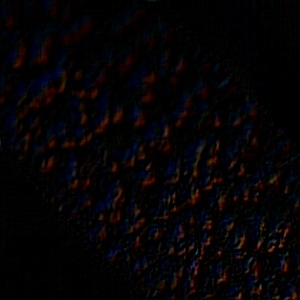
\includegraphics[width=0.2\textwidth]{resource/2-互相关.jpg}
    }
    \subfigure[卷积]{
      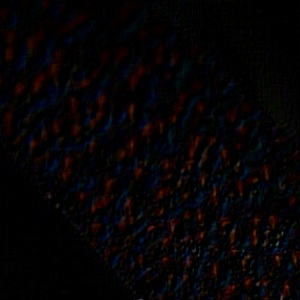
\includegraphics[width=0.2\textwidth]{resource/2-卷积.jpg}
    }
    \caption{卷积核的翻转对特征提取的影响}
    \label{Figure.Second.1}
  \end{figure}
  

  
  \subsection{\hei\xiaosan\textbf{卷积网络简介}}
    卷积网络(Convolutional Network),也叫卷积神经网络(Convolutional Neural Network,CNN),
    是一种具有局部连接、权重共享等特性的深层前馈神经网络,专门用来处理具有类似网格结构的数据的神经网络。
    

    1962年,Hubel和Wiesel通过对猫脑视觉皮层的研究,首次提出了一种新的概念——“感受野”
    (Receptive Field),对后来人工智能网络的发展起了很大的推动作用\cite{hubel1962receptive}。
    感受野是受生物学上感受野的机制而提出,在生物学上描述的是神经系统的一些神经元的特性。
    而在人工神经网络中,感受野指的是指的是卷积神经网络层输出的特征向量上的像素点对应的
    输入图像上的区域,通俗地讲,就是特征向量上的一个点对应的输入图像上的区域。1980年,Fukushima
    \cite{fukushima1982neocognitron}基于生物神经学的感受野理论提出了神经认知机和权重
    共享的卷积神经层,这被视为卷积神经网络的雏形。1989年,LeCun\cite{lecun1989backpropagation}
    将反向传播算法与权值共享的卷积神经层相结合,发明了卷积神经网络,并首次将卷积神经网络成功
    地应用到美国邮局的手写字符识别程序中。1998年,LeCun\cite{lecun1998gradient}提出了
    卷积神经网络的经典网络模型LeNet-5,它是第一个成功应用于数字\zs 识别问题的卷积神经网络。
    
 
  \subsection{\hei\xiaosan\textbf{卷积网络的特点}}
    % 卷积神经网络由神经认知机模型(Neocognitron)演变而来,由于其具有局部
    % 区域连接、权值共享、池化的结构特点,使得卷积神经网络在图像处理领域表现出色。与
    % 其他神经网络相比,卷积神经网络的特殊性表现在权值共享与局部连接等方面。权值共享使
    % 得卷积神经网络的网络结构与生物神经网络更加类似,从而更容易从中提取特征。局部连接
    % 不像传统神经网络那样,两个相连的网络层之间只有部分神经元互相连接,这两个特点很大
    % 程度上降低了网络模型的复杂度,减少了参数的数目,也提高了整个神经网络的训练效率。
    卷积运算通过三个重要的思想帮助改进深度学习系统:稀疏交互(Sparse Interactions)、
    参数\zs 共享(Parameter Sha\zs reing)和等变\zs 表示(Equivariant Represe\zs ntations)。
    
    稀疏交互的本质是对全连接的规避,这是通过使核的大小远小于输入的大小来达到的。当处理一
    张图像时,输入的图像可能包含几十万个像素点,但是我们可以使用只有数十个像素点的卷积核来
    达到提取特征的目的。这意味着我们不仅可以存储更少的参数,而且还大大减少了计算量,提高了
    统计效率。稀疏交互的图形化表示如图\ref{Figure.Second.2}所示。
    \begin{figure}[htbp]
      \centering
      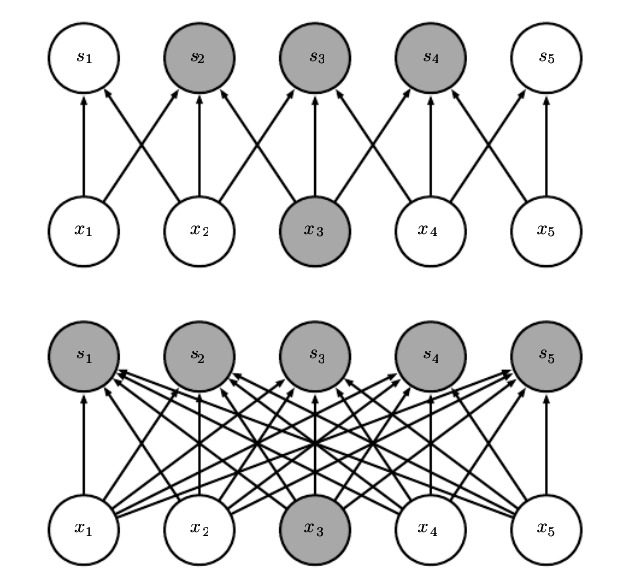
\includegraphics[width=.4\textwidth, natwidth=624, natheight=577]{resource/2.3-sparse.png}
      \caption{稀疏交互}
      \label{Figure.Second.2}
    \end{figure}
    
    参数共享是指在一个模型的多个函数中使用相同的参数。在传统的神经网络中,当计算一层的
    输出时,权重矩阵的每一个元素只使用一次,当它乘以输入的一个元素之后就再也用不到了。
    在卷积神经网络中,核的每一个元素都作用在输入的每一个位置上。参数\zs 共享保证了我们只需\zs 
    要学习一个参数\zs 集合,而不是每一个\zs 位置都需要学习一个新的\zs 集合。因此,卷积在存储需求和
    统计效率方面极大地优于稠密矩阵的乘法运算。

    在处理图像\zs 数据时,卷积产生\zs 了一个二维\zs 映射来表明某些特\zs 征在输入中出现的位\zs 置。
    如果我们移动输入中的图像,它的表示也会在输出中移动同样的量,这种性质就叫做等变表示。
    对于卷\zs 积来说,参数共\zs 享的特殊形式使\zs 得神经网络\zs 层具有对平移\zs 等变的性质。如果一个函数满足\zs 
    输入改变,输\zs 出也以同样的方式改\zs 变这一性质,我们\zs 就说它是等\zs 变的。特别的,如果函数$f(x)$与
    $g(x)$满\zs 足$f(g(x))=g(f(x))$,我们就说$f(x)$对于变换$g$具有等\zs 变性。对于卷积来说,
    如果令$g$是输\zs 入的任意平移函数,那么卷积\zs 函数对于$g$具有等变性。

  
  \subsection{\hei\xiaosan\textbf{卷积网络的结构}}
    卷积\zs 网络一般由数个卷\zs 积层(Convolu\zs tional layer)、池化层\zs (Pooling 
    layer)、全连\zs 接层及输出层交叉堆叠而成,卷积层和池化层一般会取多个,采用卷积层和
    池化层交替堆叠的模式。卷积层并\zs 行地计算多个卷积产生一组线性\zs 激活响应,每一个线性激活\zs 响应
    将会通过一个非线\zs 性的激活函数,例如整流\zs 线性激活函数。然后使用池\zs 化层来进一步调\zs 整这一层的输出。
    最后添加0~2个全连接层。
    目前,整个网络结构趋向于使用更小的卷积核(比如11和33)以及更深的网络结构。
    此外,由于卷积的操作性越来越灵活,池化层的作用也变得越来越小,因此目前比较流行的卷积网络中
    池化层的比例也越来越低,趋向于全卷积网络。
    
   
